\subsubsection{无处不在的噪声}
上一章我们把图像和标定参数接起来了，不过目标的位置并不会因此变得安安静静。同一个装甲板，连续几帧解出来的坐标可能在抖；车一加速，按匀速模型预测的位置也可能跟不上。这时候你大概会想：能不能把这些跳动抹平一点？可以，不过我们先分清跳动从哪里来，不然滤波器很可能只是把错误画得更好看。

过程噪声（process noise）描述当前运动模型没解释的变化，比如匀速模型没有写进去的加速度。观测噪声（measurement noise）描述测量相对真实量的误差，比如角点定位、量化或读出扰动。分类取决于你定义的状态和模型，不是见到“机器人抖”就一定写进 Q、见到“算法跳”就一定写进 R。固定零偏、单位错误和错误点序，也不能直接当成零均值随机噪声糊过去。

\begin{example}[先把两种误差拆开]
模型预测位置 1.0 m，目标因突然加速到了 1.2 m，而传感器读到 1.18 m。模型未解释的变化是 0.2 m，测量误差是 $-0.02$ m。前者提醒我们检查运动模型，后者提醒我们检查观测；它们都可能出现在同一帧里。
\end{example}
\begin{exercise}\label{ex:v2-filter-bias}
真实位置不变，传感器却持续偏移 0.1 m。你会先查什么？说明为什么增加平滑程度不一定能修好它。
\end{exercise}

\subsubsection{先看平滑，再看它付出的代价}
滤波（filtering）按模型和观测提取我们需要的信息。它可以抑制某些频率，也可以估计状态；但“更平滑”“噪声更小”“更准确”不是可以互换的三个词。尤其是追踪运动目标时，旧数据拖住输出，你看到的平滑曲线可能已经落后于目标。

\begin{example}[均值很稳，也可能跟错位置]
先看四个观测 9、11、9、11，真值为 10，平均正好是 10。现在目标移动到 15，最后一个观测也变为 15：
\begin{tpython}
observed = [9., 11., 9., 15.]
average = sum(observed)/len(observed)
assert average == 11.
print(average, average-15.)  # 输出 11 和 -4
\end{tpython}
计算没有错，但窗口里还留着三个旧位置。不能因为输出不抖，就说它已经跟上了目标。
\end{example}
\begin{exercise}\label{ex:v2-filter-window}
把最后一次观测改为 15，计算窗口均值与最新真值的差。若缩短窗口，跟随与抑噪通常怎样变化？
\end{exercise}

\paragraph*{低通、高通和滑动窗口}
一阶低通（low-pass）常写成
\[
y_k=a z_k+(1-a)y_{k-1},\qquad 0<a\le1.
\]
$a$ 小一些，保留的历史多一些，通常更平滑，也跟得更慢；$a=1$ 就完全使用当前输入。固定 $a$ 时，实际采样间隔改变也会改变以秒计的响应，别把一个“好用的系数”搬到所有帧率。

滑动平均取最近一段数据的均值，本章只用当前与过去样本，不偷偷访问未来帧。图像中的高斯卷积也能平滑，但空间像素滤波与时间序列滤波的轴不同。高通（high-pass）则抑制低频成分，比如从当前输入中减去低通分量，保留变化较快的部分；减完不是把目标真值提取出来，它也会保留高频噪声。按需设计频率响应与抗混叠，不能靠调一个系数补回采样前已混叠的信息。

\begin{example}[给平滑加上可观察的输入]
完整项目在本卷 \path{examples/filter/state-estimation-demo}。先从数值数组开始，再将同一运动轨迹交给 KF、EKF、UKF；生成数据都有明确真值，暂时不接实车。我们使用 Ubuntu 的系统 Python：
\begin{tbash}
sudo apt install python3-numpy python3-matplotlib
cd /你的教材目录/02-专项技术栈/examples/filter/state-estimation-demo
\end{tbash}
把路径换成实际位置。目录里各文件分别承担下面的事情：
\begin{tbash}
state-estimation-demo/
  smooth.py         # 因果低通、尾部均值、高通
  fusion.py         # 独立或相关的标量融合
  linear.py         # 预测、矩阵更新、协方差检查
  scalar.py         # 一维手算结果的运行入口
  data.py           # 同一轨迹与模拟观测
  run.py            # KF/EKF 与 UKF 序列比较
  sigma.py          # 取点和统计量重建
  moments_demo.py   # 线性精确/非线性近似对照
  ukf.py            # 完整预测与观测更新
  plot.py           # 读取实际数组画图
  README.md
\end{tbash}
首先看 \path{smooth.py}，初始低通输出为 0，窗口在开头只平均已有样本：
\lstinputlisting[numbers=left,language=Python,basicstyle=\footnotesize\ttfamily,firstline=1,lastline=22]{examples/filter/state-estimation-demo/smooth.py}
随后用种子42给“前50个为0、随后100个为1”的阶跃加标准差0.2的高斯扰动，保存实际数组。高通由输入减低通得到，两者相加应还原输入：
\lstinputlisting[numbers=left,language=Python,basicstyle=\footnotesize\ttfamily,firstnumber=23,firstline=23]{examples/filter/state-estimation-demo/smooth.py}
\begin{tbash}
python3 smooth.py --alpha 0.2 --window 10 --output out/smooth
python3 smooth.py --alpha 1 --window 10 --output out/current
\end{tbash}
通用形式是 \texttt{python3 smooth.py [选项]}。alpha 控制低通，window 是尾部窗口长度，output 选择新输出目录，同名文件会写入。本次 alpha=0.2 的低通 RMSE 约0.120，原始观测约0.171，但无噪声阶跃要到第11次更新才达到90\%；alpha=1 第一次就到达，代价是没有低通抑噪。这两个指标回答不同问题。
\end{example}
\begin{figure}[htbp]
\centering
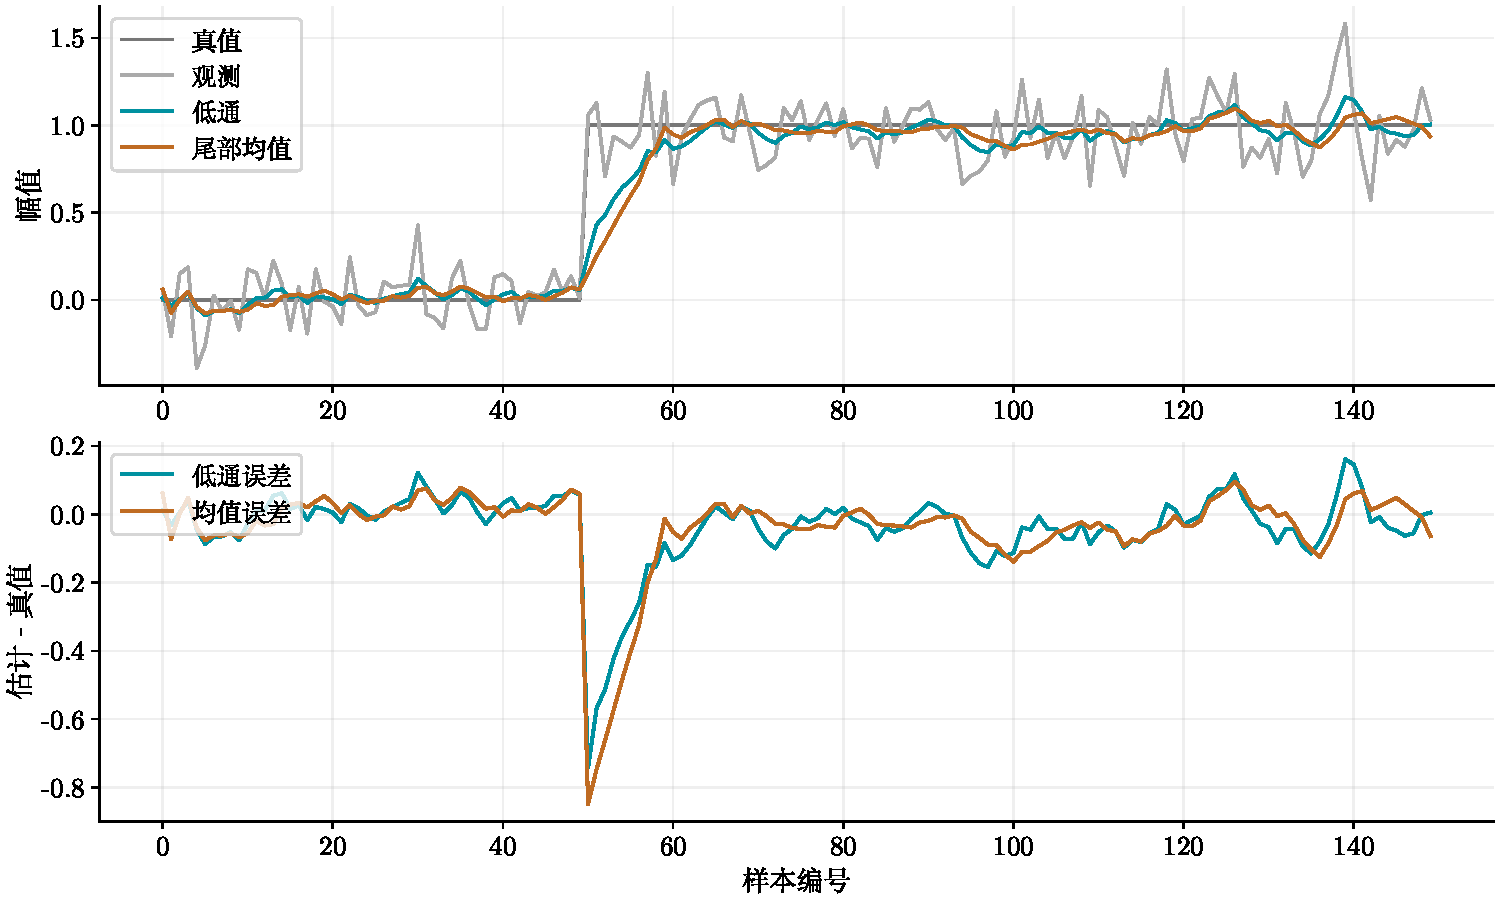
\includegraphics[width=.94\textwidth]{images/filter_smooth_revised.pdf}
\caption{实际保存的模拟序列：阶跃后的偏差与整段误差一起看，不能只挑静止部分}
\label{fig:v2-filter-smooth}
\end{figure}
\begin{exercise}\label{ex:v2-filter-lowpass}
对连续输入1、初值0，手算 $a=0.2$、0.5、1 的前三步。运行各变体，记录达到无噪声阶跃90\%的更新次数，解释与整段 RMSE 的区别。
\end{exercise}
\begin{conclusion}
先确定你想保留的信号，再决定平滑方式。尾部窗口和递归低通都可能跟随滞后；高通保留快速变化也可能保留噪声。至少同时看真值误差与变化后的响应，输出方差变小不是单独的合格证。
\end{conclusion}

\subsubsection{从两份估计推到融合权重}
卡尔曼滤波（Kalman Filter，KF）看上去有一堆矩阵，不过它的更新可以先从两份估计讲起。假设 $X=p+N_1$、$Y=p+N_2$ 都无偏，噪声均值为0，方差分别为 $\sigma^2,\tau^2$，先假定彼此独立。我们用
\[
\hat p=wX+(1-w)Y
\]
融合，均值仍为 $p$；方差为 $w^2\sigma^2+(1-w)^2\tau^2$。对 $w$ 求导并令其为0，得到
\[
w=\frac{\tau^2}{\sigma^2+\tau^2},\qquad
\operatorname{Var}(\hat p)=\frac{\sigma^2\tau^2}{\sigma^2+\tau^2}.
\]
这就是逆方差加权：越不确定的那份估计，权重越小。高斯分布并不是“任何噪声都长这样”，这里方差推导只需要上述二阶统计与独立条件。

如果两份结果来自同一张图，它们可能共享误差。记交叉协方差为 $c=\operatorname{Cov}(N_1,N_2)$，则
\[
\operatorname{Var}(\hat p)
=w^2\sigma^2+(1-w)^2\tau^2+2w(1-w)c,\qquad
w=\frac{\tau^2-c}{\sigma^2+\tau^2-2c}.
\]
最后一个分母为正时才按此求唯一最优权重。完全相同、等方差的噪声使分母为0，重复平均不会增加信息。某些相关条件下最优权重还可能超出0--1，不要拿独立情形的直觉硬套。

\paragraph*{从信号功率再看一次*}
若共同信号为 $s(t)$，两路零均值噪声与它及彼此不相关，$s_1=s+N_1,s_2=s+N_2$，那么
\[
E[s_1s_2]=E[s^2],\qquad
E[(ws_1+(1-w)s_2)^2]
=E[s^2]+w^2\sigma^2+(1-w)^2\tau^2.
\]
共同信号保留，噪声功率按权重变化，仍得到前面的结论。独立性不会让交叉项凭空多出两份噪声方差；如果噪声相关，就重新加入 $2w(1-w)c$。

\begin{example}[真的把相关性算进去]
\path{fusion.py} 使用方差与相关系数 $\rho$ 得到 $c=\rho\sqrt{\sigma^2\tau^2}$，并完整计算融合方差：
\lstinputlisting[numbers=left,language=Python,basicstyle=\footnotesize\ttfamily]{examples/filter/state-estimation-demo/fusion.py}
\begin{tbash}
python3 fusion.py
python3 fusion.py --v2 1 --rho 0
python3 fusion.py --v2 1 --rho 1
\end{tbash}
默认两估计2/4、方差1/3，输出权重0.75、均值2.5、方差0.75。两方差都为1且独立，方差变为0.5；完全正相关时仍为1。最后一条主要检查统计公式的退化情况：等方差、完全相同的无偏噪声在实际同一次采样中应给出相同读数，不能拿代码固定的2/4当这种联合分布的有效样本。
\end{example}
\begin{exercise}\label{ex:v2-filter-fusion}
将第二个方差改为1，算均值与独立融合方差；再令 $\rho=1$，解释为何不能把同一帧派生的两份信息当成两次独立测量。
\end{exercise}

\subsubsection{状态、协方差和预测：把“小滑块”写进程序}
真实追踪不一定有两个传感器，不过我们还有上一时刻的估计。假设一个小滑块沿直线运动，短时间内速度近似不变，用状态 $\boldsymbol x=[p,v]^T$ 记录位置和速度，单位为 m 与 m/s：
\[
F=\begin{bmatrix}1&\Delta t\\0&1\end{bmatrix},\qquad
H=\begin{bmatrix}1&0\end{bmatrix}.
\]
$F$ 把速度换成这段时间的位置变化，$H$ 只取位置作为观测。只测位置不等于速度永远不可估，连续位置及运动模型提供了时间约束；但约束是否足够还要检查系统可观性。
\begin{figure}[htbp]
\centering
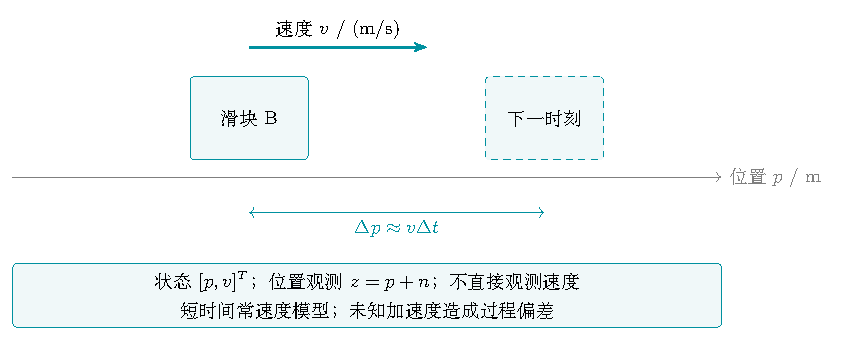
\includegraphics[width=.9\textwidth]{images/filter_motion_revised.pdf}
\caption{沿一维方向运动的小滑块：位置观测配合时间模型估计速度}
\label{fig:F_filter-1}
\end{figure}
更一般的状态与观测可写成
\[
\boldsymbol x_k=F_k\boldsymbol x_{k-1}+B_k\boldsymbol u_k+\boldsymbol w_k,\qquad
\boldsymbol z_k=H_k\boldsymbol x_k+\boldsymbol n_k.
\]
控制输入可省略，本项目不把未知真实加速度当作已知控制。过程噪声 $\boldsymbol w_k$ 协方差为 $Q_k$，观测噪声 $\boldsymbol n_k$ 协方差为 $R_k$；我们先采用零均值、加性并与先前误差相应独立的模型。时间戳要决定实际 $\Delta t$，乱序、丢帧和不规则采样不能一直装作每次都是0.1秒。

\paragraph*{协方差不是一排“可信度分数”}
二维协方差写成
\[
P=\begin{bmatrix}\sigma_p^2&c_{pv}\\c_{pv}&\sigma_v^2\end{bmatrix}.
\]
对角线是各分量方差，非对角线是协方差；$P_{pp}$ 的单位是 m$^2$，$P_{vv}$ 是 (m/s)$^2$，$P_{pv}$ 是 m$^2$/s，不能都写成同一个无单位小数。矩阵须对称半正定，负方差不能解释成“特别有信心”。对独立随机向量，和的协方差相加；相关时还要加交叉协方差及其转置。线性变换满足
\[
E[A\boldsymbol x]=AE[\boldsymbol x],\qquad
\operatorname{Cov}(A\boldsymbol x)=A P A^T.
\]
因此预测不只推进均值，还传播误差：
\begin{equation}
\boldsymbol x_k^-=F_k\boldsymbol x_{k-1}^++B_k\boldsymbol u_k,\qquad
P_k^-=F_kP_{k-1}^+F_k^T+Q_k.
\label{eq:Px}
\end{equation}
上标减号表示看到新观测之前，称先验（prior）；加号表示更新之后，称后验（posterior），不是给状态加减一个常量。

相关系数 $\rho=c_{pv}/(\sigma_p\sigma_v)$ 在方差非零时位于 $[-1,1]$。它不是椭圆短长轴之比，也不是协方差非对角线的乘积。零相关、等方差的联合高斯等密度线是圆；方差不同就可能是轴对齐椭圆。一般分布中零相关也不保证独立。
\begin{figure}[htbp]
\centering
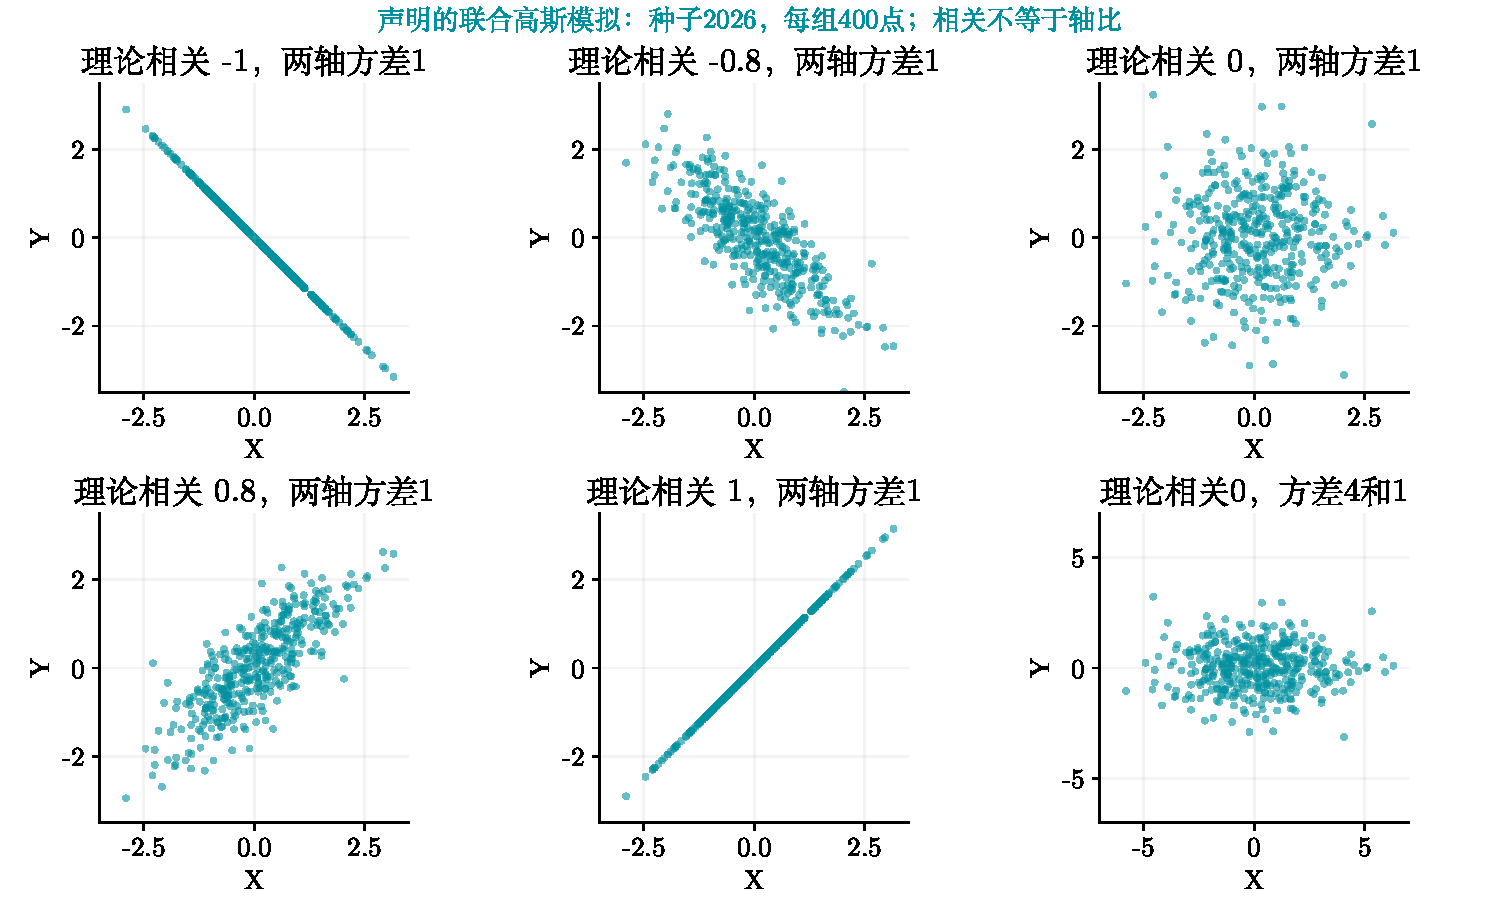
\includegraphics[width=.94\textwidth]{images/filter_covariance_revised.pdf}
\caption{明确生成条件的相关性示意；右下零相关但两轴方差不同，不是圆}
\label{fig:related}
\end{figure}

\begin{example}[给 Q 一个能核对单位的模型]
本项目假定每段内有一个未知、零均值的加速度扰动，方差为 $q_a$，令
\[
G=\begin{bmatrix}\Delta t^2/2\\\Delta t\end{bmatrix},\qquad
Q=q_aGG^T.
\]
这是离散“每段一个随机加速度”的模型，不是连续白噪声谱密度公式；两者的 $q$ 单位和时间幂次不同。$\Delta t=0.1$ s、$q_a=0.5$ (m/s$^2$)$^2$ 时，
\[
Q=\begin{bmatrix}0.0000125&0.00025\\0.00025&0.005\end{bmatrix}.
\]
下面项目的 run 正是按此生成 Q，不直接给位置和速度各塞一个相同方差。R=0.04 m$^2$ 对应位置标准差0.2 m。
\end{example}
\begin{exercise}\label{ex:v2-filter-covariance}
写出上述 F、H、Q 的尺寸和各项单位。把 $\Delta t$ 改为0.05 s，计算新的 Q，解释为何不能只改 F 而沿用原 Q。
\end{exercise}

\subsubsection{Kalman 更新：先比较观测，再修正状态}
看到新位置后，我们先问“它和模型预期差多少”，而不是去求 $H^{-1}$。H 往往是长方形，根本没有普通逆矩阵。创新量（innovation）和它的协方差为
\[
\boldsymbol r_k=\boldsymbol z_k-H_k\boldsymbol x_k^-,
\qquad S_k=H_kP_k^-H_k^T+R_k.
\]
然后将创新映回状态空间：
\begin{align}
K_k&=P_k^-H_k^TS_k^{-1},\\
\boldsymbol x_k^+&=\boldsymbol x_k^-+K_k\boldsymbol r_k.
\label{eq:final}
\end{align}
$P_k^-$ 为 $n\times n$，H 为 $m\times n$，S 为 $m\times m$，所以 K 为 $n\times m$。这一维位置观测可以同时修正位置和速度，靠的是预测后两者的协方差联系。在标量 H=1 的情形，R 变小通常增大对观测的权重；矩阵 K 的各项不能都当作0--1的置信度。

\paragraph*{为什么是这个增益*}
令误差为“估计减真值”，更新后有 $\boldsymbol e^+=(I-KH)\boldsymbol e^-+K\boldsymbol n$。先验误差与观测噪声不相关时，后验协方差为
\[
P^+=(I-KH)P^-(I-KH)^T+KRK^T.
\]
这称 Joseph 形式。对 $\operatorname{tr}(P^+)$ 关于 K 求导，得到
\[
\frac{\partial\operatorname{tr}(P^+)}{\partial K}
=-2P^-H^T+2K(HP^-H^T+R).
\]
令其为0就回到前面的增益。如果 S 可逆，在精确运算中还能化为 $P^+=(I-KH)P^-$；实际程序保留 Joseph 形式，有助于减轻浮点误差破坏对称性和非负性的风险。矩阵求解不必显式构造逆，更不能用逐元素除法假装矩阵逆。

\begin{example}[把预测和更新写完整]
\path{linear.py} 检查协方差，再预测；更新时用 \texttt{solve} 解线性方程，最后算完整 Joseph 形式。末尾对称化只消除微小浮点不对称，遇到明显负特征值仍报错，不靠“加个数”掩盖模型错误：
\lstinputlisting[numbers=left,language=Python,basicstyle=\footnotesize\ttfamily]{examples/filter/state-estimation-demo/linear.py}
\path{scalar.py} 把它接成原来的手算例：随机游走、初值0、P=1、Q=0.1、R=0.9、第一次观测2。
\lstinputlisting[numbers=left,language=Python,basicstyle=\footnotesize\ttfamily]{examples/filter/state-estimation-demo/scalar.py}
\begin{minipage}{\linewidth}
\begin{tbash}
python3 scalar.py
python3 scalar.py --r 9
\end{tbash}
\end{minipage}
先验方差1.1，默认 K=0.55、更新状态1.1、方差0.495；改R=9时 K约0.108911，状态约0.217822，方差约0.980198。这里只改假定观测方差，其余完全一样，才能解释权重为什么改变。
\end{example}
\begin{exercise}\label{ex:v2-filter-scalar}
手算 R=9 的 K、状态与方差，再与程序核对。说明 Q、R、P 分别属于哪里，为什么不能交换预测与更新的顺序。
\end{exercise}
\begin{figure}[htbp]
\centering
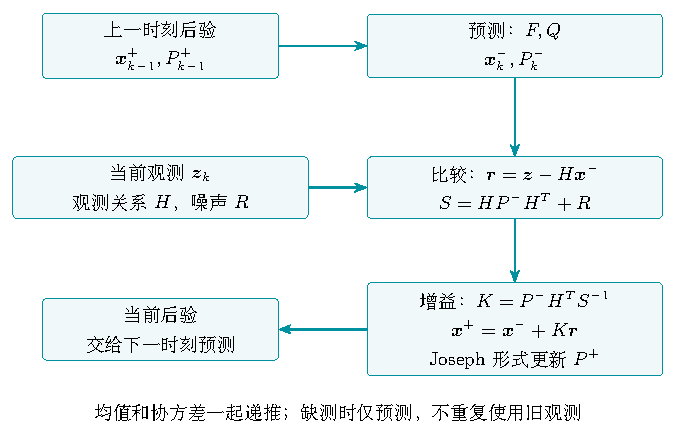
\includegraphics[width=.94\textwidth]{images/filter_flow_revised.pdf}
\caption{上一时刻后验先预测，再与当前观测比较；同时推进均值和协方差}
\label{fig:kalman}
\end{figure}
\begin{conclusion}
KF 更新的是状态估计及其误差协方差，并没有拿到每一步真实误差。先用 F/Q 预测，再用 H/R 与新观测更新；P 描述当前估计不确定性，S 描述创新不确定性。在线性、零均值且满足相应不相关条件时，KF 给出最优线性估计；联合高斯条件下对应最小均方误差估计。模型、单位或偏置错了，漂亮的矩阵也救不了。
\end{conclusion}

\subsubsection{把一步手算接成一段轨迹}
前面的一步很容易算对，不过追踪还要面对持续运动、加速和缺测。先看 \path{data.py}：起点1 m、速度0.3 m/s，中间三分之一施加0.7 m/s$^2$加速度，其他时段为0；观测加标准差0.2 m的噪声。真实加速度用于生成真值，不传给滤波器。位置与斜距使用同一份噪声，方便后面比较，不拿它们当独立传感器融合。
\begin{example}[同一输入同时跑两种估计]
\lstinputlisting[numbers=left,language=Python,basicstyle=\footnotesize\ttfamily]{examples/filter/state-estimation-demo/data.py}
\path{run.py} 先规定模式、时间和方差，再逐步执行预测/更新。linear 直接观测位置，range 则观测斜距；UKF 的实现稍后完整展开。
\lstinputlisting[numbers=left,language=Python,basicstyle=\footnotesize\ttfamily,firstline=1,lastline=29]{examples/filter/state-estimation-demo/run.py}
接下来给 UKF 相同初值，准备输出数组，再进入逐帧循环。当一帧缺测，只预测，P 仍继续传播；有观测时计算创新与归一化创新平方 $\mathrm{NIS}=r^2/S$。本项目只观测一个标量，向量观测则使用 $\boldsymbol r^TS^{-1}\boldsymbol r$，不能逐项随意除。
\lstinputlisting[numbers=left,language=Python,basicstyle=\footnotesize\ttfamily,firstnumber=30,firstline=30]{examples/filter/state-estimation-demo/run.py}
\begin{tbash}
python3 run.py --mode linear --output out/linear
python3 run.py --mode linear --q 0 --output out/q0
python3 run.py --mode linear --drop-every 5 --output out/drops
\end{tbash}
dt 单位秒；q 为每段加速度方差，r 为观测方差；bias 给观测加固定偏置，seed 决定随机数据，drop-every=5 每五帧跳过一次更新，alpha 属于后面的无迹变换。默认150步，本次 KF 位置 RMSE约0.1385 m；丢帧变体跳过30次更新。Q=0表示我们假定匀速模型没有过程不确定性，但模拟目标仍会加速，看看输出在这段怎样落后。

程序保存真值、观测、估计、创新和 NIS，并记录全过程的协方差最小特征值。这里的特征值是当前状态坐标下的数值检查，换单位会改变数值，不能把它当跨单位的物理评分。NIS 均值约1可以作标量模型下的检查线索，但不能凭一次小样本的平均值就确认模型正确；还要看创新的均值、相关性、变化时段和参数假设。
\end{example}

\begin{example}[用保存的数组画图]
\path{plot.py} 只读前面输出，不在画图时重算滤波。它默认使用教材已有中文字体，也可通过 --font 指定字体文件：
\lstinputlisting[numbers=left,language=Python,basicstyle=\footnotesize\ttfamily]{examples/filter/state-estimation-demo/plot.py}
\begin{tbash}
python3 plot.py --input out/smooth/series.npz --output out/smooth.pdf
python3 plot.py --input out/linear/series.npz --output out/linear.pdf
\end{tbash}
滤波曲线、真值误差和创新分开看。若想改变参数，先运行 run 保存新数组，再绘图；不要只改图上的标签。
\end{example}
\begin{figure}[htbp]
\centering
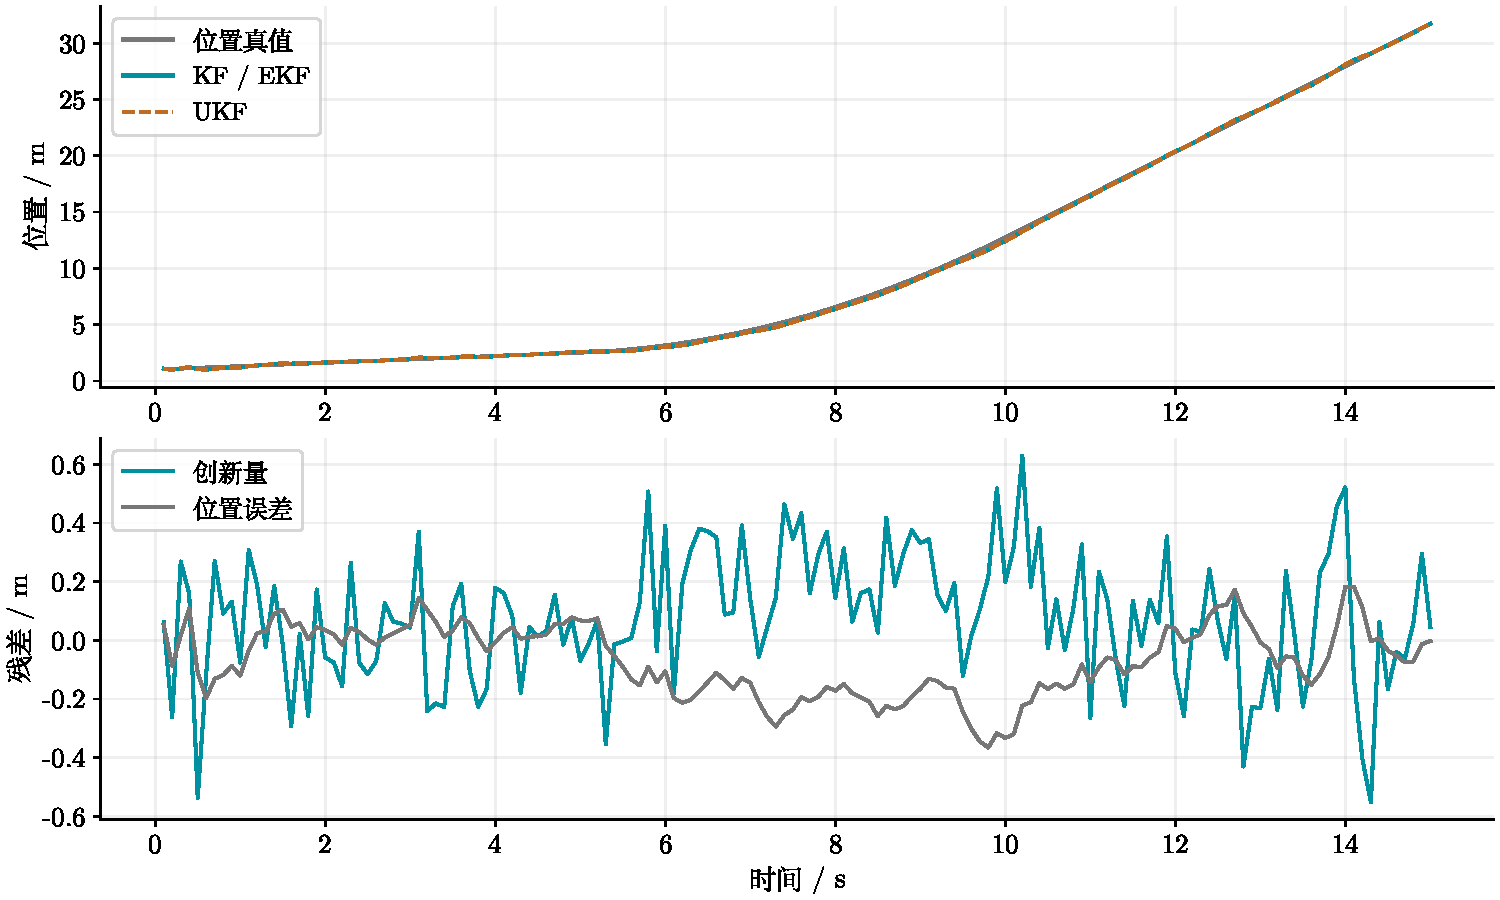
\includegraphics[width=.94\textwidth]{images/filter_track_revised.pdf}
\caption{实际模拟轨迹的 KF/UKF 输出与创新；线性模式下两者结果几乎重合}
\label{fig:v2-filter-track}
\end{figure}
\begin{exercise}\label{ex:v2-filter-track}
分别运行默认、Q=0、R=0.4 和缺测变体，用独立目录保存。记录 RMSE、NIS、协方差最小特征值与加速段表现；再加入0.5 m偏置，说明为什么平滑不能保证无偏。项目准备、状态模型与序列运行在这道综合练习中一起核对。
\end{exercise}

\subsubsection{非线性观测：EKF 线性化的是哪里}
如果观测直接是位置，H 只是取一个分量；若测的是距离，事情就不同了。设传感器与运动轨道垂直间距固定为2 m，水平位置为 p，斜距观测为
\[
h(\boldsymbol x)=\sqrt{p^2+2^2}.
\]
这不是把位置乘一个常量能得到的关系。距离也不能单独区分 $p$ 与 $-p$；本实验给定正侧轨道及初始状态，不宣称解决了全局符号歧义。

扩展卡尔曼滤波（Extended Kalman Filter，EKF）对均值使用实际非线性函数，对误差传播使用局部雅可比。一般加性模型为 $\boldsymbol x_k=f(\boldsymbol x_{k-1})+\boldsymbol w_k$、$\boldsymbol z_k=h(\boldsymbol x_k)+\boldsymbol n_k$；观测函数的输入是状态，不是拿观测 z 自己喂自己。预测雅可比 $F_k$ 在上一时刻后验处求，观测雅可比 $H_k$ 在当前先验处求。本项目过程仍线性，观测雅可比为
\[
H_k=\begin{bmatrix}p^-/\sqrt{(p^-)^2+4}&0\end{bmatrix}.
\]
创新用 $z-h(\boldsymbol x^-)$，不能改成 $z-H_k\boldsymbol x^-$；雅可比不是原函数。随后用这个 H 传播创新协方差与增益，状态按原函数的创新更新。

\begin{example}[用同一份 run 检查 EKF]
run 中 range 分支正是先计算 h，再求 H，把 h 的结果作为 update 的 expected。执行：
\begin{tbash}
python3 run.py --mode range --output out/range
python3 plot.py --input out/range/series.npz --output out/range.pdf
\end{tbash}
默认条件下本次 EKF 位置 RMSE约0.1535 m，UKF约0.1568 m。这个实验中 UKF 没有更准，名字更高级不等于当前模型一定更好。接近 p=0 时距离的一阶位置导数很小，局部更新较弱；初值错误、模型歧义或很大不确定性都会影响求解。
\end{example}
\begin{exercise}\label{ex:v2-filter-ekf}
在 p=1 m处计算 h 与 H 的非零项，手算 $h(1.001)-h(0.999)$ 的差分导数并比较。指出 EKF 创新中为什么必须保留 h；描述 p=0 时的局部约束问题。
\end{exercise}

\subsubsection{无迹变换：传播几个点，再重建统计量}
局部线性化会漏掉曲率的影响。我们保留原来的例子：$X\sim U(-1,1)$，$Y=X^2+X$。由 $E[X]=0$、$E[X^2]=1/3$、$E[X^4]=1/5$ 得
\[
E[Y]=\frac13,\qquad
\operatorname{Var}(Y)=\frac15+\frac13-\frac19=\frac{19}{45}.
\]
在0处的一阶近似却是 $Y\approx X$，给出均值0、方差1/3。问题并不在乘法写错，而在“先取均值再过函数”通常不等于“过函数后取均值”。

无迹变换（Unscented Transform，UT）换一种思路：用少量确定选择的 sigma 点匹配均值与协方差，将点送进真实函数，再按权重重建统计量。它不是 Monte Carlo 的随机采样，也不保证有限个点能准确描述任意非线性或任意分布的高阶矩。

\paragraph*{取点与权重要一起看}
对于 n维、正定协方差P，NumPy 的 Cholesky 分解给出下三角 L，使 $P=LL^T$。取点使用 L 的列；如果你换成上三角因子，就要相应换方向。常见缩放 UT 定义
\[
\lambda=\alpha^2(n+\kappa)-n,\qquad c=n+\lambda>0.
\]
用 $L_cL_c^T=cP$ 得到
\begin{equation}
\chi_0=\boldsymbol x,\qquad
\chi_i=\boldsymbol x+(L_c)_{:i},\qquad
\chi_{n+i}=\boldsymbol x-(L_c)_{:i},\quad i=1,\ldots,n.
\label{eq:sigma}
\end{equation}
两侧是相反方向，缩放包含平方根，不能把 $(n-\lambda)L$ 当作另一半点。均值与协方差权重分别为
\[
W_0^{(m)}=\frac{\lambda}{c},\quad
W_0^{(c)}=\frac{\lambda}{c}+1-\alpha^2+\beta,\quad
W_i^{(m)}=W_i^{(c)}=\frac1{2c}.
\]
非中心点的分子是1，不是 $\lambda$。$\alpha$ 控制展开尺度，$\kappa$ 配合维度缩放，$\beta$ 纳入分布先验；高斯输入常用 $\beta=2$，不代表所有分布都具有高斯四阶矩。参数可能产生负权重，取很小 alpha 还可能放大浮点消减误差；本项目默认 alpha=1、kappa=0、beta=2，不把它说成通用最优值。Cholesky 要求正定，半正定奇异矩阵需要专门处理，不能一概声称所有协方差都可直接分解。

\begin{example}[重建后再说取点正确]
\path{sigma.py} 将 L 的各列变为行排列的点，\texttt{moments} 重建均值与协方差：
\lstinputlisting[numbers=left,language=Python,basicstyle=\footnotesize\ttfamily]{examples/filter/state-estimation-demo/sigma.py}
\path{moments_demo.py} 首先重建非对角协方差，再传播仿射函数，最后回到均匀分布的非线性例子：
\lstinputlisting[numbers=left,language=Python,basicstyle=\footnotesize\ttfamily]{examples/filter/state-estimation-demo/moments_demo.py}
\begin{tbash}
python3 moments_demo.py
\end{tbash}
重建原均值[1,2]与协方差后，仿射结果应等于 $A\boldsymbol x+b$ 和 $APA^T$。非线性例中，这组 UT 得到均值1/3，却得到方差5/9，仍不同于均匀分布真值19/45；输出同时给出20万次声明的随机抽样对照。这恰好说明匹配前两阶统计量并不足以指定所有高阶矩。不能只展示这次均值对了，就宣布 UKF 对任何函数都准确。
\end{example}
\begin{figure}[htbp]
\centering
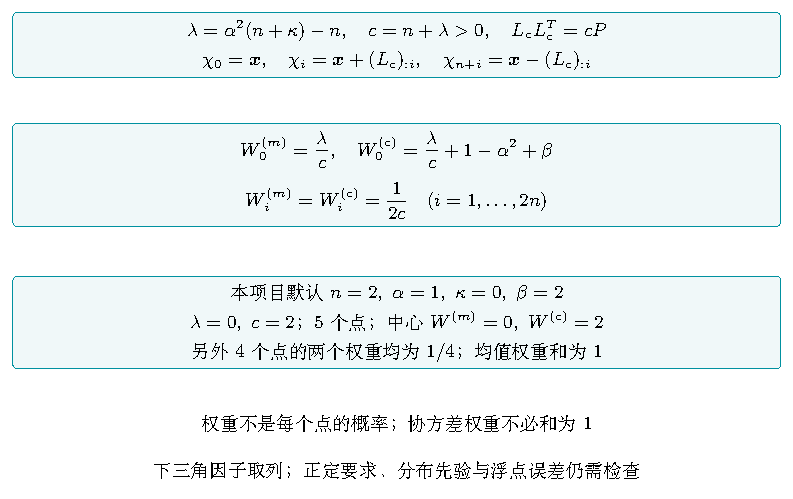
\includegraphics[width=.94\textwidth]{images/filter_weights_revised.pdf}
\caption{缩放 UT 的点、权重与默认二维数值；中心均值权重0也仍需保留中心协方差权重}
\label{fig:weight}
\end{figure}
\begin{exercise}\label{ex:v2-filter-ut}
用现有 sigma 点传播 $y=2x+1$，计算均值与方差，与线性公式比较。再核对均匀输入 $X^2+X$ 的精确方差与本次 UT 方差，解释两种结论为什么可以同时成立。
\end{exercise}

\subsubsection{UKF：把无迹变换接回预测与更新}
无迹卡尔曼滤波（Unscented Kalman Filter，UKF）把前面的取点、传播、重建接成递归估计。本项目采用独立加性过程/观测噪声：先将点过状态函数得到先验均值与协方差，加 Q，再基于完整先验重新取点、传播观测。重新取点是为了让观测统计也包含过程噪声；本章没有展开非加性噪声的增广状态版本。

记先验观测均值为 $\bar z$，状态和观测的离差为 $\delta x_i,\delta z_i$，则
\[
P_{xz}=\sum_i W_i^{(c)}\delta x_i\delta z_i^T,\qquad
S=P_{zz}=\sum_i W_i^{(c)}\delta z_i\delta z_i^T+R,
\]
\begin{equation}
K=P_{xz}S^{-1},\qquad
\boldsymbol x^+=\boldsymbol x^-+K(\boldsymbol z-\bar z),\qquad
P^+=P^--KSK^T.
\label{eq:ukf-K}
\end{equation}
矩阵时仍是求解，不是分子分母逐元素相除。本项目仅一个标量观测，所以 S 是标量；代码的 \texttt{cross/S} 在这个限定下才是正确运算。

\begin{example}[完整 UKF 和两种模式的对照]
\lstinputlisting[numbers=left,language=Python,basicstyle=\footnotesize\ttfamily]{examples/filter/state-estimation-demo/ukf.py}
\begin{tbash}
python3 run.py --mode linear --output out/linear
python3 run.py --mode range --alpha 0.3 --output out/range-a03
\end{tbash}
默认线性模式下 KF 与 UKF 的全过程状态最大差约 $9.8\times10^{-15}$，是浮点量级；这支持取点、Q传播与更新在此模型下相符。range 模式就不要求两者相同，也不承诺 UKF 总能胜出。缺测时两个程序只返回预测，收到下一帧再更新，不能将旧观测反复当作新的独立信息。
\end{example}
\begin{exercise}\label{ex:v2-filter-ukf}
n=2、alpha=1、kappa=0、beta=2时计算 lambda、点数、中心及其他权重。运行 linear/range 及 alpha=0.3 变体，记录状态差、RMSE和协方差；解释为何需要先加 Q 再取观测点。
\end{exercise}
\begin{conclusion}
KF 直接传播线性统计量，EKF 传播均值与局部雅可比，UKF 传播选定点。三者都需要正确模型、单位和噪声假设。把重建、仿射传播、创新、误差和协方差连起来检查，既不因为曲线抖就一味调 R，也不因为名字里带“最优”就省略验证。
\end{conclusion}
\begin{note}
线性 KF 与 EKF 的经典介绍可查 Welch 与 Bishop 的
\href{https://www.cs.utexas.edu/~pstone/Courses/393Rfall15/readings/Welch+Bishop-TR-95.pdf}{An Introduction to the Kalman Filter（大学课程镜像）}；
缩放无迹变换和 UKF 见 Wan 与 van der Merwe 的
\href{https://groups.seas.harvard.edu/courses/cs281/papers/unscented.pdf}{The Unscented Kalman Filter for Nonlinear Estimation}。
先按本章小例子把尺寸和统计量算通，再阅读一般系统与增广噪声版本。
\end{note}
